% ----------------------------------------------------------
% ILLUSTRATIVE EXAMPLE
% ----------------------------------------------------------
\section{Illustrative Example}

To illustrate the behavior of \UD, consider an entity evaluated over twelve
intervals. Table~\ref{tab:ud_example} reports realized demand $y_t$, forecasted
demand $\yhat_t$, and the resulting shortfall depth
$s_t = \pospart{y_t - \yhat_t}$ for each interval.

% ----------------------------------------------------------
% TABLE: UD EXAMPLE
% ----------------------------------------------------------
\begin{table}[h!]
\centering
\begin{tabular}{c c c c}
\hline
Interval $t$ & $y_t$ & $\yhat_t$ & Shortfall Depth $s_t$ \\
\hline
1  & 20 & 22 & 0 \\
2  & 28 & 25 & 3 \\
3  & 32 & 29 & 3 \\
4  & 35 & 36 & 0 \\
5  & 40 & 37 & 3 \\
6  & 42 & 45 & 0 \\
7  & 38 & 34 & 4 \\
8  & 30 & 31 & 0 \\
9  & 26 & 22 & 4 \\
10 & 24 & 27 & 0 \\
11 & 22 & 23 & 0 \\
12 & 18 & 19 & 0 \\
\hline
\end{tabular}
\caption{Example of realized demand, forecasts, and shortfall depths for a single
entity evaluated over twelve intervals.}
\label{tab:ud_example}
\end{table}

Shortfalls occur in intervals 2, 3, 5, 7, and 9, with corresponding depths of
$3$, $3$, $3$, $4$, and $4$. The resulting Underbuild Depth is therefore
\[
\UD
=
\frac{3 + 3 + 3 + 4 + 4}{5}
=
3.4.
\]

This value indicates that, conditional on underbuilding occurring, the forecast
underestimates demand by an average of 3.4 units. Intervals in which forecasted
demand meets or exceeds realized demand do not contribute to the metric.

Figure~\ref{fig:ud_depths} visualizes the distribution of shortfall depths across
intervals for this example. The dashed horizontal line indicates the value of
\UD, highlighting the average severity of underbuilding relative to individual
shortfall events.

% ----------------------------------------------------------
% FIGURE: UD SHORTFALL DEPTHS
% ----------------------------------------------------------
\begin{figure}[h!]
\centering
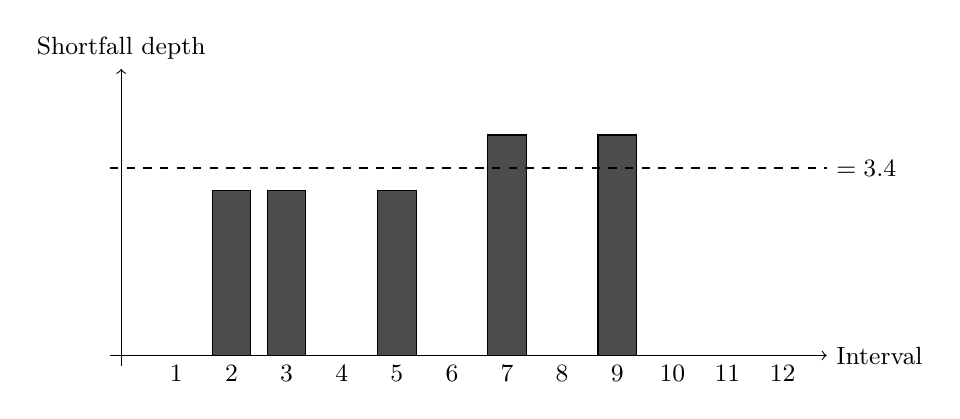
\begin{tikzpicture}[scale=0.7]

% Axes
\draw[->] (-0.2,0) -- (12.8,0) node[right] {\small Interval};
\draw[->] (0,-0.2) -- (0,5.2) node[above] {\small Shortfall depth};

% Shortfall bars (only intervals with s_t > 0)
\draw[fill=black!70] (2-0.35,0) rectangle ++(0.7,3);
\draw[fill=black!70] (3-0.35,0) rectangle ++(0.7,3);
\draw[fill=black!70] (5-0.35,0) rectangle ++(0.7,3);
\draw[fill=black!70] (7-0.35,0) rectangle ++(0.7,4);
\draw[fill=black!70] (9-0.35,0) rectangle ++(0.7,4);

% Interval labels
\foreach \t in {1,...,12} {
    \node[below] at (\t,0) {\small \t};
}

% Dashed UD line
\draw[dashed] (-0.2,3.4) -- (12.8,3.4);
\node[right] at (12.8,3.4) {\small $\UD = 3.4$};

\end{tikzpicture}
\caption{Shortfall depths across intervals for the example in
Table~\ref{tab:ud_example}. The dashed line indicates the Underbuild Depth (\UD).}
\label{fig:ud_depths}
\end{figure}